\section{PAL ABI performance}


%The efficiency of \hostapis{} directly impacts the performance of \graphene{} on each host.
%A large portion of \linuxapis{} inside \thelibos{} require resources or abstractions from the host OS.
%Since \thehostabi{} is the only interface for requesting host OS features,
%the definition of \thehostabi{}
%restricts the options for a \picoproc{} to optimize its own performance, according to the application's performance patterns.
%Although each PAL may optimize individual \hostapi{} for general circumstances,
%all applications must share the same PAL ABI and thus tolerate the same overheads of exporting these \hostapis{} on each host.



The section evaluates the performance of \thehostabi{} in comparison with
the underlying host \linuxapis{}.
The PAL ABI implementation depends on the existing system interfaces,
which partially determines the latency of each \hostapi{} 
%Upon a certain host, the base latency of a \hostapi{} is mostly determined by the host \linuxapis{} or abstractions
%chosen to implement such \hostapi{}.
%Three primary factors determine the efficiency of \hostapis{}.
%First, especially on Linux or other monolithic OS,
%most of \thehostabi{} are directly translated to similar \linuxapis{}.
%The efficiency of these \hostapis{}
%are dominated by the basic cost of the host system interface,
%and the performance of corresponding \linuxapis{}.
For instance, on the Linux PAL, the latency of \palcall{StreamRead} is comparable to the latency of \syscall{read},
since the former is mostly just
a wrapper of the latter.
If a \picoproc{} runs inside an SGX enclave,
the cost of enclave exits will increase
the latency of \hostapis{},
including the cost of copying data between enclave and untrusted memory.
%invoking a \syscall{read} \linuxapi{}, and returning the contents back to the enclave.
%The latency on the SGX PAL is then mostly dominated by the overheads
%of switching the context between the enclave
%and the untrusted, external PAL using SGX instructions,
%and bringing memory into the EPC (enclave page cache).
% or decrypting memory on a last-level cache miss.


In theory, the definition of \thehostabi{}
is meant to minimize the translation cost to most host system interfaces,
by adopting similar, UNIX-like semantics.
%Since most \hostapis{} are just wrappers
%of the underlying \linuxapis{},
%the translation cost is mostly reduced to simply replacing the generic identifiers and control flags
%to the semantics that are recognized by the host OS.
A major cost
in translation is to parse a URI (unified resource identifier)
for determining the file path or network address
%and compose a equivalent file system path or network address
to request host OS services.
%The second factor is the translation cost
%of the \hostapis{}.
%For portability, \thehostabi{} is defined with generic semantics, without host-specific notions
%such as process identifiers, file descriptors,
%file system paths,
%and \linuxapi{} flags.
%The PAL must translate the arguments of \hostapis{}, including PAL handles, URIs (Uniform Resource Identifiers), and generic flags,
%to the arguments interpretable by the host kernel.
Other translation costs,
such as converting optional flags,
are relatively marginal, compared with the overall latency of a \hostapi{}.
%because the translation is mostly straightforward,
%and only requires simply logics
%and little memory copy.
%Without extra security checks,
%a \hostapi{} is more likely to suffer high overheads if the implementation
%requires additional \linuxapis{} for complementary operations
%to the base abstraction,
%or constantly retrying a \linuxapis{} at failures.



More significant overheads
on a few \hostapis{} contribute to security checks or enforcements,
to protect applications
inside host-specific threat models.
%for ensuring the safety of running an application
%within the threat model
%of a host.
%Finally, the third factor that impacts the PAL call efficiency
%is the cost of security checks,
%either inside the host kernel or the guest.
%The cost of security checks varies between hosts, and is correlated with the presumed security models.
For example, the threat model on a Linux host
focuses on the attacks between mutually-untrusting applications via system interfaces;
therefore,
the security checks on the Linux PAL
restrict the sharing of host resources and block \linuxapis{} that are not required by the Linux PAL.
%using both the reference monitor and \seccomp{} filter.
In another threat model, with the SGX enclave, 
security checks for each \hostapi{}
protects the application and \libos{} against malicious inputs from an untrusted OS,
%and thus focus on validating the results of \linuxapis{},
using either cryptographic techniques or semantic checks.
%Cryptographic techniques are used to: (1) validate the file against the secure hash, at \palcall{StreamOpen}, (2) check the file chunks against a Merkle tree of hash values, at \palcall{StreamRead}, and (3) establish a TLS connection over inter-enclave RPC, at \palcall{ProcessCreate}.
On the SGX PAL, the latency of a \hostapi{} may be dominated
by security checks,
especially the ones based on cryptographic operations.
%on large chunks of data exported to the untrusted OS.


The evaluation in this section is based on micro-benchmark programs similar to \lmbench{} 2.5~\cite{McVoy:lmbench}.
For each \hostapis{}, the evaluation also shows the breakdowns
of its latency or throughput,
by benchmarking the PALs both with and without the security mechanisms, such as the \seccomp{} filter and reference monitor on the Linux PAL,
as well as testing under different
implementation strategies.
The evaluation focuses on \hostapis{} that are especially sensitive for the performance of the \graphene{} \libos{}.


% the efficiency of \hostapis{} on both Linux and SGX hosts, and shows the impact of each performance factor.
%The evaluation is based on micro-benchmark programs similar to \lmbench{} 2.5~\cite{McVoy:lmbench},
%and is compared against
%similar \linuxapis{} on Linux.



\subsection{Stream I/O}
\label{sec:eval:pal:stream}

This section separate the evaluation of stream I/O in \thehostabi{} into 
%The \hostapis{} for stream I/O can be separated into 
two categories:
(1) file system operations and (2) I/O operations on a network socket or a RPC stream.
The evaluation for file system operations
primarily measures
the latency of retrieving file metadata from the storage or a host kernel file system directory cache,
as well as the latency of sequential reads or writes
inside a regular file.
%access a UNIX-style, hierarchical, host file system,
%with either random access to file contents,
%or access to file attributes (metadata).
The evaluation for other I/O streams, such as a network socket or a RPC stream,
then focuses on measuring the latency or bandwidth
of sending and receiving messages 
across \picoprocs{} or applications.

%over a network address or a local, in-kernel queue.
%Due to the difference in the nature of these operations,
%the evaluation separates
%file access from network or RPC workloads.






\paragraph{Opening a file.}
Similar to \syscall{open} in a Linux process,
the latency of \palcall{StreamOpen} to open a host file
is correlated with the length and depth
of file paths request,
as shown in Figure~\ref{fig:eval:pal:open-latency} (a).
%The evaluation shows the latency of identifying a file inside the host storage and attaching the file resources to the running application. 
%Figure~\ref{fig:eval:pal:open-latency} (a) and (b) shows the latency of \palcall{StreamOpen} on the Linux and SGX PALs,
%in comparison with \syscall{open} in a native Linux process.
The experiment
measures the latency of repeatedly opening a file,
which does not include the latency of retrieving the file attributes from the disk.
%and shows simply the efficiency
%of retrieving the file metadata cached inside the host OS.
Without disk I/O cost,
the latency of \syscall{open}
%or other file-searchig \linuxapis{} (e.g., \syscall{stat})
in a native Linux process is dominated by lookup time inside the Linux file system directory cache,
and is proportional to the number of components in the path~\cite{tsai15dcache}.
%shows that, with a warm cache,
%the latency of a file-searching \linuxapi{} on Linux,
%such \syscall{open} or \syscall{stat}, 
%is strictly correlated with
%lengths and depths of the requested paths,
%because the lookup functions of the current file system directory cache design
%are based on searching each path components
%(i.e., directory names separated by the common slash character)
%inside a hash table.
%The latency of \palcall{StreamOpen} on the Linux PAL
%shows the same pattern.
%Figure~\ref{fig:eval:pal:latency} (a)
%shows a similar pattern for \palcall{StreamOpen}
%on the Linux PAL,
%because \syscall{open} is used as the underlying host \linuxapi{}. %of \palcall{StreamOpen}.
The latency of \palcall{StreamOpen} on the Linux PAL includes the latency of \syscall{open},
with additional cost for translating a URI
to the corresponding file path.
The benchmark result shows this overhead to be around
6--10\%.
The \seccomp{} filter, with the BPF JIT (Just-in-time) optimization,
adds an additional \roughly{}0.9 \usec{},
or 7--10\% overhead to the latency.
Finally, enabling the reference monitor
adds 14-21\% overhead.
The overhead of reference monitor
contributes to comparing the file path against
the sandbox rules
inside the kernel module,
and thus is correlated with path length.


\begin{figure*}[t!]
\centering
\footnotesize
\resizebox{\textwidth}{!}{%
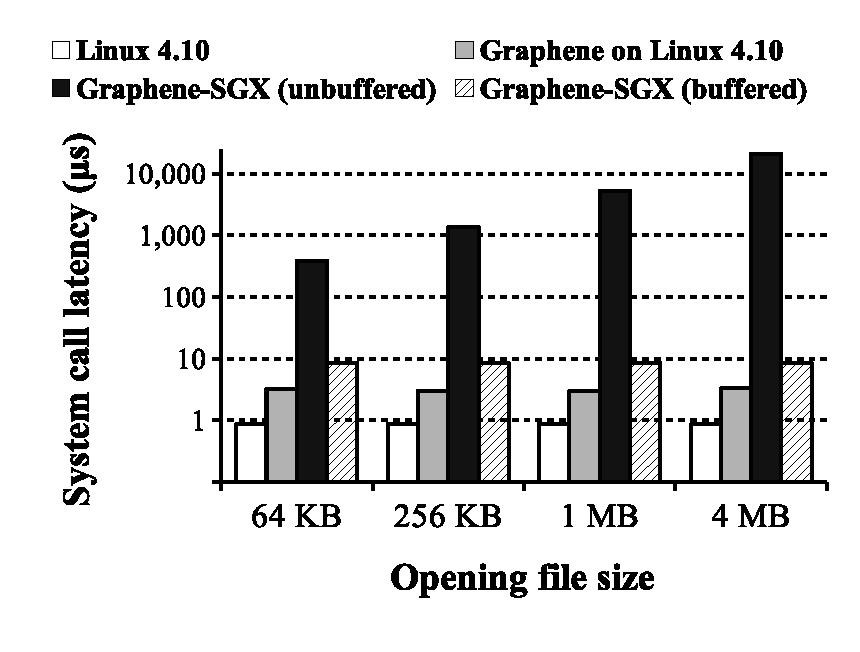
\includegraphics[height=10em]{pal/open-latency}
\quad
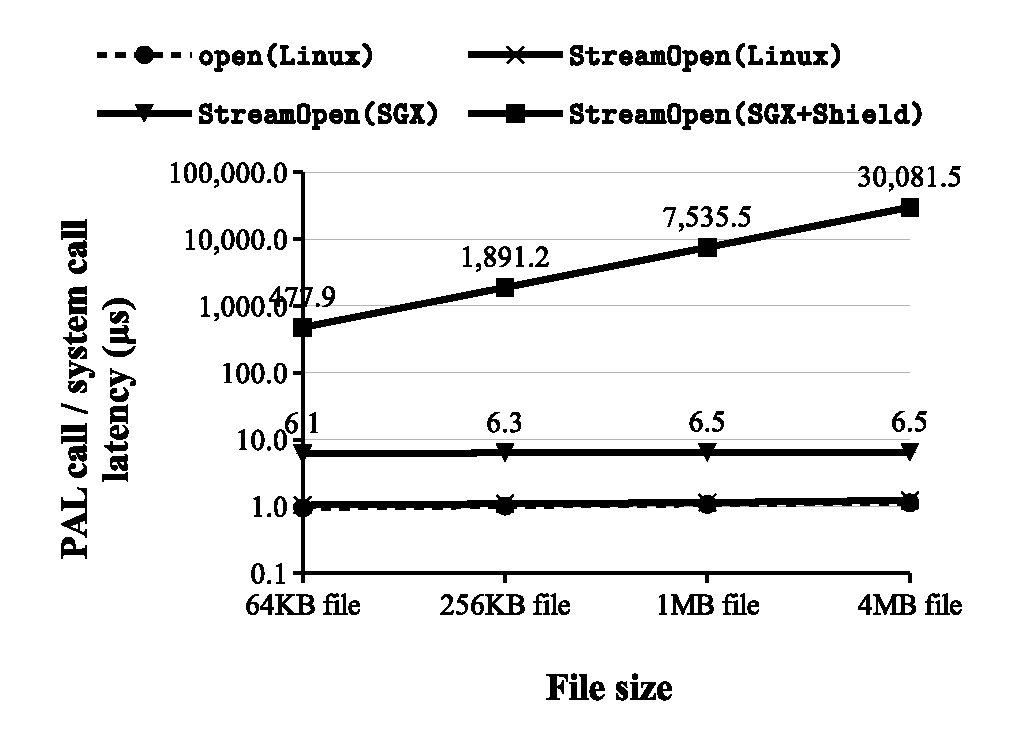
\includegraphics[height=10em]{pal/sgx-open-latency}
}
\parbox{0.49\textwidth}{\centering\bf (a) Linux vs. Linux PAL}
\parbox{0.49\textwidth}{\centering\bf (b) Linux vs. Linux PAL vs. SGX PAL}
\caption{Latency of \palcall{StreamOpen} on the Linux PAL  and SGX PAL, versus \syscall{open} on Linux.
Lower is better.
Figure (a) compares \palcall{StreamOpen} on the Linux PAL,
with and without a \seccomp{} filter ({\bf +SC})
and reference monitor ({\bf +RM}), against \syscall{open} on Linux. Figure (b) compares \palcall{StreamOpen} on a SGX PAL,
with and without integrity checks ({\bf +CHK}),
against the Linux PAL and \syscall{open} on Linux.}
\label{fig:eval:pal:open-latency}
\end{figure*}


Opening a file on the SGX PAL
imposes significant overheads for verifying
the integrity of file contents.
Figure~\ref{fig:eval:pal:open-latency} (b) shows the latency of \palcall{StreamOpen} inside of an SGX enclave, versus the latency on the Linux PAL
and in a native Linux process.
Without any security checks to shield the guest from the untrusted OS,
the latency of \palcall{StreamOpen} is dominated by the overhead of exiting the enclave and copying the argument, such as the file paths, out of the enclave.
The overheads of unshielded \palcall{StreamOpen} is 4.7--5.5$\times$, or \roughly{}5 \usec{}.
If a file is shielded with integrity protection,
\palcall{StreamOpen} will verify the checksum of the whole file against the manifest, and generate a Merkel Tree of file chunk hashes
for optimizing the latency of following \palcall{StreamRead} or \palcall{StreamMap}.
The overhead of enforcing the integrity check is correlated with the file size, and dominated by the time of
calculating a SHA256 hash of the file.
For a 4MB file, the latency of \palcall{StreamOpen} can be up to \roughly{}30 \msec{}.









\paragraph{File reads and writes.}
The latency of file reads and writes on the Linux PAL
is close to
\syscall{read} and \syscall{write}
in a Linux process.
Figure~\ref{fig:eval:pal:read-write-latency} (a) and (b) compare the latency of sequential reads and writes 
on the Linux PAL and Linux,
and show almost no overheads on the Linux PAL.
%On the Linux PAL,
%the latency of sequential reads and writes
%is correlated
%with the size of file access,
%when the size is larger than the 4KB page size.
%Besides, the latency of sequential writes is up to twice of the latency of sequential reads,
%due to the reading and writing speeds
%of the host storage.
%The latency of 
%\palcall{StreamRead} and \palcall{StreamWrite}
%on the Linux PAL
%shows a similar patterns:
%the latency is close to \syscall{read} or \syscall{write} with the size,
%with marginal overheads especially when
%the size is larger than 4KB.
The \seccomp{} filter adds a fixed overhead
around 0.06--0.09 \msec{},
which is marginal to the overall latency.
Enabling the reference monitor has nearly no overheads,
since the reference monitor only checks file paths at \palcall{StreamOpen}.
 


\begin{figure*}[t!]
\centering
\footnotesize
\resizebox{\textwidth}{!}{%
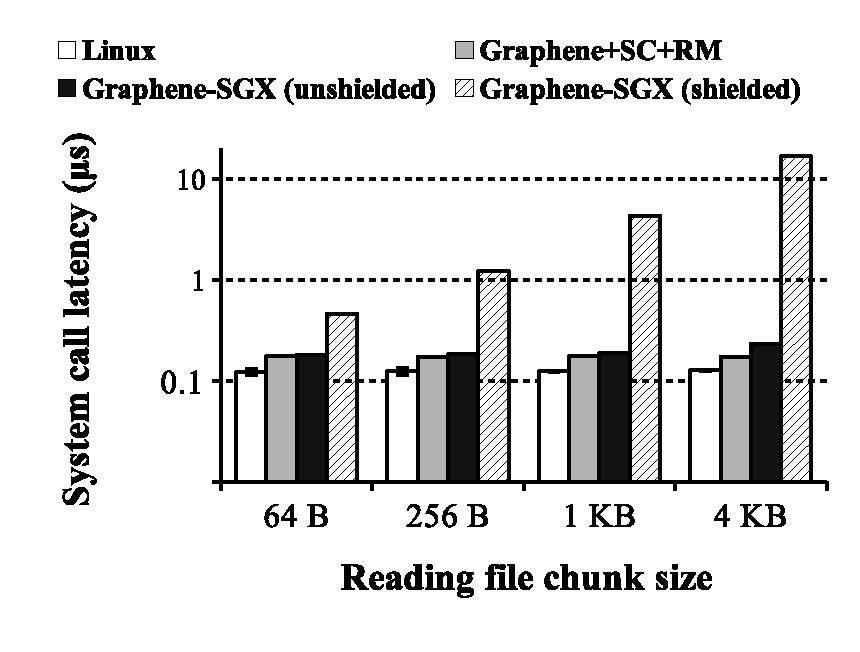
\includegraphics[height=10em]{pal/read-latency}
\quad
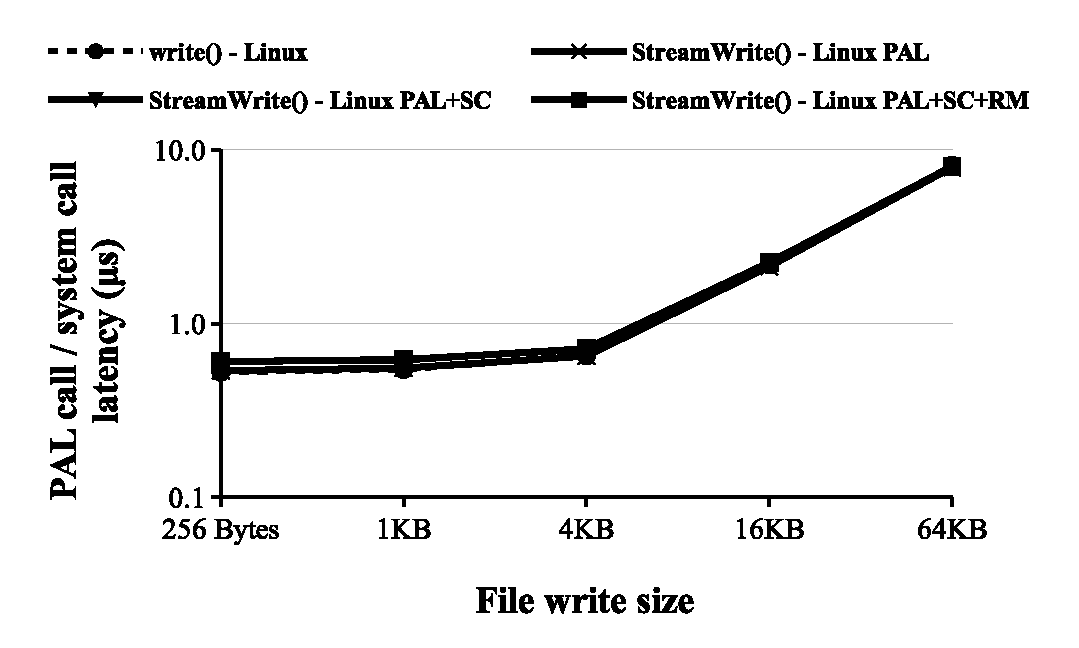
\includegraphics[height=10em]{pal/write-latency}
}
\parbox{0.49\textwidth}{\centering\bf (a) Sequential read}
\parbox{0.49\textwidth}{\centering\bf (b) Sequential write}
\caption{Latency of sequential \palcall{StreamRead} and \palcall{StreamWrite} on the Linux PAL,
versus \syscall{read} and \syscall{write} on Linux.
Lower is better.
Figure (a) and (b) respectively compares \palcall{StreamRead} and \palcall{StreamWrite} on the Linux PAL,
with and without a \seccomp{} filter ({\bf +SC})
and reference monitor ({\bf +RM}), against \syscall{read} and \syscall{write} on Linux.}
\label{fig:eval:pal:read-write-latency}
\end{figure*}

\begin{figure*}[t!]
\centering
\footnotesize
\resizebox{\textwidth}{!}{%
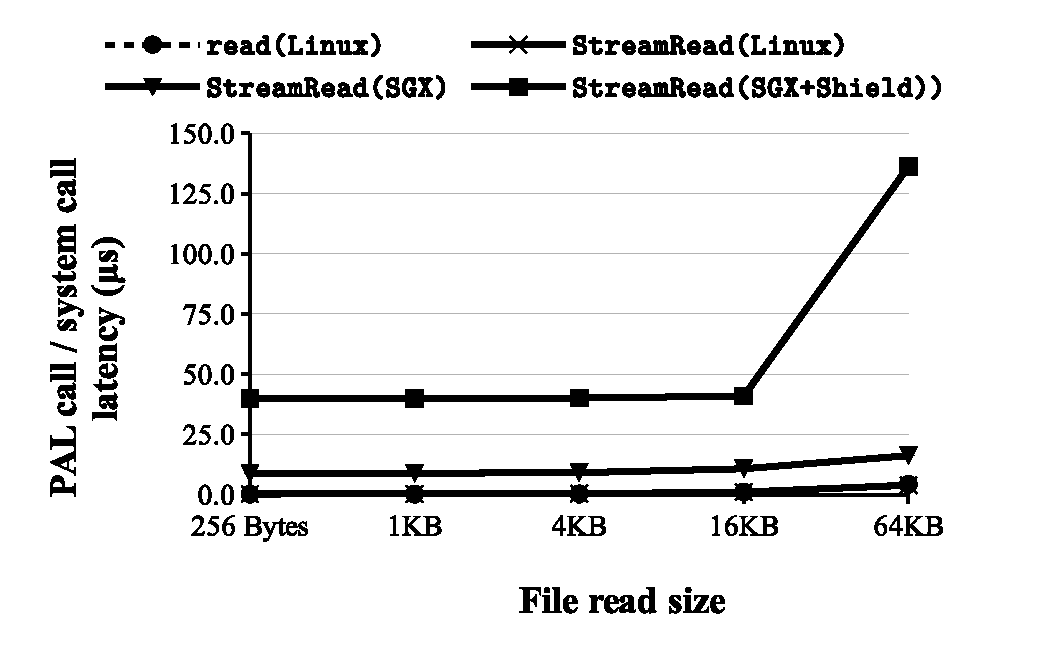
\includegraphics[height=10em]{pal/sgx-read-latency}
\quad
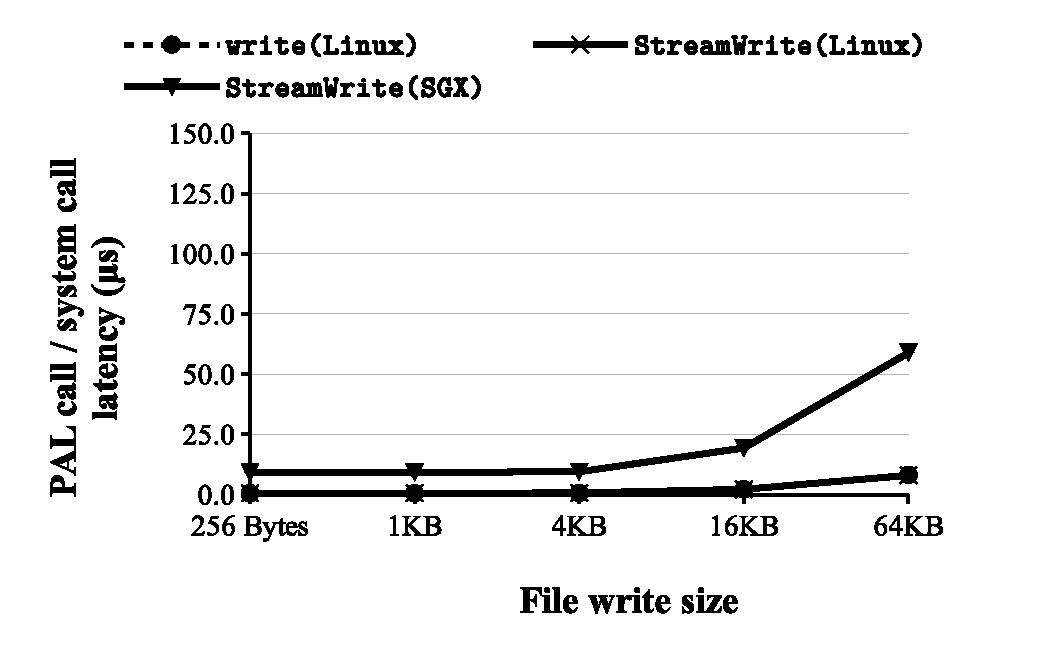
\includegraphics[height=10em]{pal/sgx-write-latency}
}
\parbox{0.49\textwidth}{\centering\bf (a) Sequential read}
\parbox{0.49\textwidth}{\centering\bf (b) Sequential write}
\caption{Latency of sequential \palcall{StreamRead} and \palcall{StreamWrite} on the SGX PAL,
versus the Linux PAL and Linux.
Lower is better.
Figure (a) and (b) respectively compares \palcall{StreamRead} and \palcall{StreamWrite} on the SGX PAL,
with and without integrity checks ({\bf +CHK})
and reference monitor ({\bf +RM}), against the Linux PAL and \syscall{read} and \syscall{write} on Linux. The current design does not support integrity checks for \palcall{StreamWrite}.}
\label{fig:eval:pal:sgx-read-write-latency}
\end{figure*}


On the SGX PAL,
as shown in
Figure~\ref{fig:eval:pal:sgx-read-write-latency} (a) and (b), both sequential reads and writes
have significant overheads over the latency on Linux or the Linux PAL.
The overheads contribute to:
(1) copying the contents between the enclave and the untrusted PAL; (2) cryptographic operations for 
integrity checks. Without any integrity checks,
the cost of exiting the enclave
and copying the contents across the enclave boundary is
8--12 \usec{} for reads and 8--50 \usec{} for writes.
If the SGX PAL checks the integrity of file contents
at file reads,
the latency is bounded by
the cost of copying 16KB blocks into the enclave
and calculating the secure hashes to compare with the Merkle tree.
Reducing the hashing size from 16KB to even smaller block
will improve
the latency of small reads,
but also will increase the size of Merkle tree.
The experiment does not measure the overhead of integrity protection on file writes
because the feature is not yet implemented
in the SGX PAL.








%\paragraph{Network connections.}



\begin{figure*}[t!]
\centering
\footnotesize
\resizebox{\textwidth}{!}{%
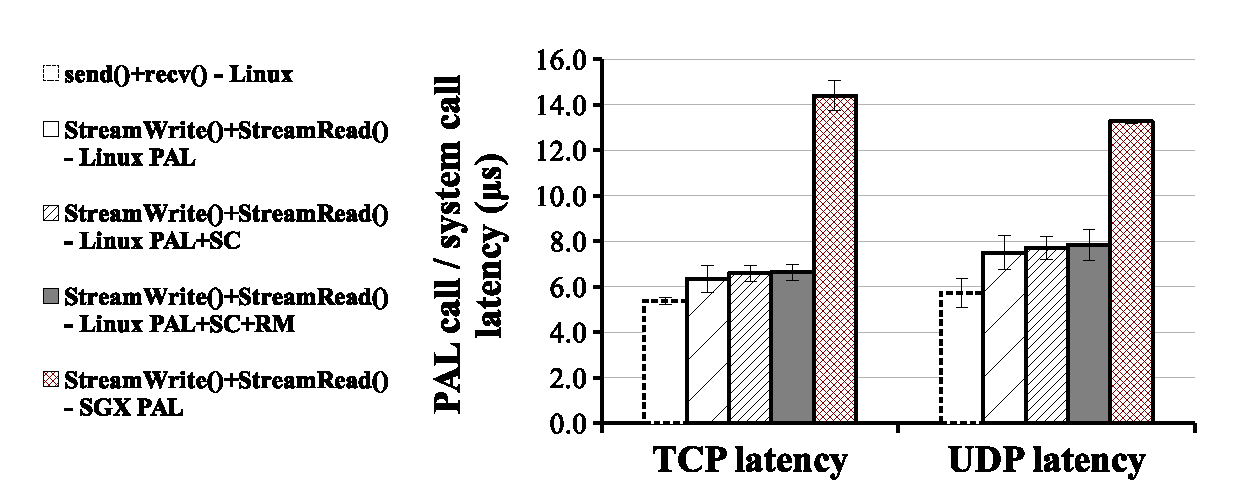
\includegraphics[height=10em]{pal/tcp-udp-latency}
\quad
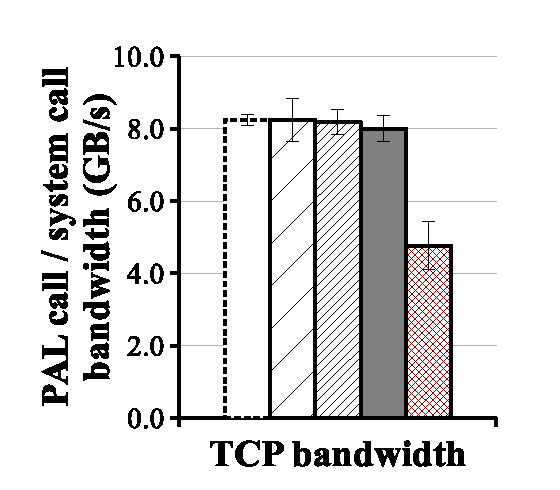
\includegraphics[height=10em]{pal/tcp-bandwidth}
}
\parbox{0.24\textwidth}{\quad}
\parbox{0.49\textwidth}{\centering\bf (a) Latency ({\usec})}
\parbox{0.24\textwidth}{\centering\bf (b) Bandwidth (MB/\asec{})}
\caption{(a) Latency of sending a short message over TCP and UDP sockets (lower is better), and (b) bandwidth of sending large data over TCP (higher is better).
The comparison is between (1) \syscall{recv} and \syscall{send} on Linux; (2) \palcall{StreamRead} and \palcall{StreamWrite} on a Linux PAL, with and without a \seccomp{} filter ({\bf +SC}) and reference monitor ({\bf +RM}); (3) the same \hostapis{} on the SGX PAL, without data protection.}
\label{fig:eval:pal:network-latency-bandwidth}
\end{figure*}



\paragraph{TCP and UDP sockets.}
%The evaluation shows both the latency and bandwidth of sending and receiving messages over a TCP or UDP sockets.
The Linux PAL imposes \roughly{}18\% and \roughly{}30\% overheads
on the latency of TCP and UDP sockets (bound on localhost),
respectively,
as shown in
Figure~\ref{fig:eval:pal:network-latency-bandwidth} (a).
The overheads specifically contribute
to cost of translating to \syscall{sendmsg} and \syscall{recvmsg}
in the Linux host,
which requires passing a data structure
containing buffer pointer, size, and a socket address
for UDP messaging. 
The UDP socket address is also checked by the reference monitor if enabled, adding extra overheads to the \hostapis{}.
Figure~\ref{fig:eval:pal:network-latency-bandwidth} (b)
also shows the bandwidth of TCP sockets
for sending 64KB messages locally,
which has only 4\% overheads on the Linux PAL.
In addition, both the \seccomp{} filter and reference monitor
cause less than 1\% overheads
on TCP bandwidth.



% shows the turnaround time of sending single-byte messages back and forth over a TCP or UDP stream (connected through the local loopback device), and
%Figure~\ref{fig:eval:pal:network-latency-bandwidth} (b)
%shows the bandwidth of a TCP or UDP stream
%to transfer
%64KB messages between \picoprocs{}.
%On the Linux PAL,
%the overheads of ping-ponging over TCP or UDP primarily contribute to the translation cost between
%the \hostapis{} to Linux \linuxapis{} (specifically, \syscall{sendmsg} and \syscall{recvmsg}),
%since the the \hostapis{} use strings as the network URIs and the Linux \linuxapis{} take a network address structure (\code{struct sockaddr}) that contains numeric representations in integers.
%The translation costs for a TCP stream and a UDP stream are \roughly{}18\% and \roughly{}30\%, respectively.
%The overhead is relatively marginal in the TCP bandwidth test,
%at \roughly{}4\%.
%Both the \seccomp{} filter and reference monitor adds
%a marginal, less than 1\% overhead
%to either the latency or bandwidth of TCP or UDP sockets.


TCP and UDP sockets on the SGX PAL
also have significant overheads compared to the Linux PAL,
due to the cost of enclave interface.
As shown in
both Figure~\ref{fig:eval:pal:network-latency-bandwidth}
(a) and (b),
the overheads of the SGX PAL on TCP and UDP latency
are \roughly{}167\% and \roughly{}131\%,
respectively; the overhead on TCP bandwidth also reaches \roughly{}79\%. 
Note that the current design
of the SGX PAL does not protect the messages sent or received
over a TCP or UDP socket.
The decision is based on previous work~\cite{osdi16scone},
which concludes that
inline encryption and authentication inside applications
is more efficient
than shielding at the enclave interface
or the system interface.
\graphenesgx{} makes the assumption
that most networked applications have adopted SSL/TLS
to protect the confidentiality and integrity of network payloads.



\begin{figure*}[t!]
\centering
\footnotesize
\resizebox{\textwidth}{!}{%
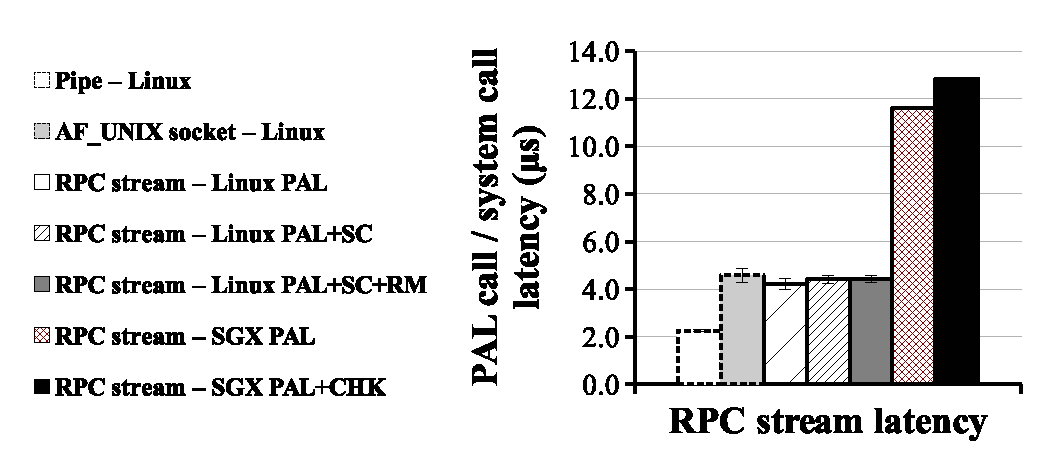
\includegraphics[height=10em]{pal/pipe-latency}
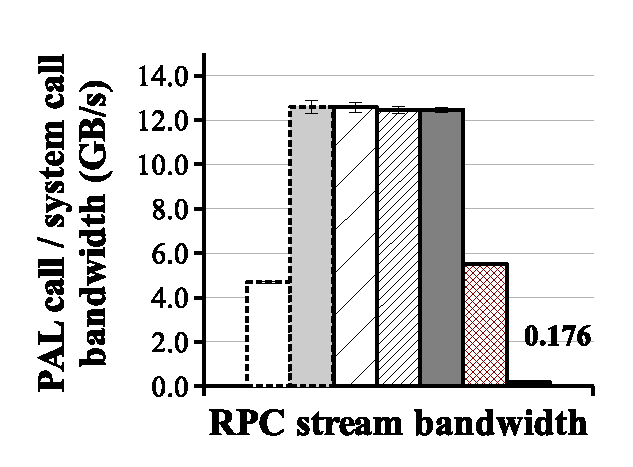
\includegraphics[height=10em]{pal/pipe-bandwidth}
}
\parbox{0.30\textwidth}{\quad}
\parbox{0.34\textwidth}{\centering\bf (a) Latency ({\usec})}
\parbox{0.34\textwidth}{\centering\bf (b) Bandwidth (MB/\asec{})}
\caption{(a) Latency of sending a short message over RPC (lower is better), and (b) bandwidth of sending large data (higher is better).
The comparison is between (1) \syscall{read} and \syscall{write} over a pipe or an AF\_UNIX socket on Linux; (2) \palcall{StreamRead} and \palcall{StreamWrite} on the Linux PAL, with and without a \seccomp{} filter ({\bf +SC}) and reference monitor ({\bf +RM}); (3) the same \hostapis{} on the SGX PAL, with and without data protection ({\bf +CHK}).}
\label{fig:eval:pal:pipe-latency-bandwidth}
\end{figure*}



\paragraph{RPC latency and bandwidth.}
%The evaluation shows the latency and bandwidth of using a RPC stream to send messages across \picoprocs{}.
Due to the implementation
of the Linux PAL,
both the latency and bandwidth
of a RPC stream on the Linux PAL is close to a UNIX domain socket
on native Linux kernel.
Figure~\ref{fig:eval:pal:pipe-latency-bandwidth} (a)
compares
the latency of sending one-byte messages
over a local RPC stream,
a pipe, and a UNIX domain socket (the last two are both in a native Linux process).
The results
show that the latency of a UNIX domain socket
is about twice as slow as a pipe,
and close to the latency of a RPC stream
on the Linux PAL,
with or without the \seccomp{} filter and reference monitor.
Figure~\ref{fig:eval:pal:pipe-latency-bandwidth} (b)
also shows the bandwidth
of messaging over a RPC stream, a UNIX domain socket,
and a pipe,
and first two reach bandwidth
more than double of the pipe bandwidth.
Both the \seccomp{} filter and reference monitor introduce marginal overheads (less than 5\%) to RPC latency and bandwidth.
Note that this performance pattern is specific
to kernels after 4.2; a zero-copy design for UNIX domain socket
is adopted in Linux 4.2,
and makes a UNIX domain socket
almost equally fast as the bulk IPC abstraction
in the Linux PAL
(see Section~\ref{sec:eval:pal:multi-proc}). 



For the SGX PAL,
the fundamental cost of enclave exits and copying message contents,
without protecting the message contents,
is \roughly{}154\% to the latency,
or \roughly{}127\% to the bandwidth.
Unlike network sockets, 
applications generally assume transferring data over a local pipe or FIFO to be secure on a trusted host, and do not enforce protection like SSL/TLS.
%\graphenesgx{} cannot assume RPC streams to be protected by SSL/TLS in applications.
%Since it is likely that an application may send sensitive information
%over a pipe or a UNIX socket,
%the underlying RPC streams must always be protected by the SGX PAL.
For each RPC stream, the SGX PAL establishes a TLS connection using a 256-bits AES-GCM algorithm, which both authenticates and encrypts the message contents.
The AES-GCM algorithm in \graphenesgx{} is accelerated by the Intel AES-NI instructions, which are guaranteed to exist on a SGX-enabled CPU.
With the hardware-accelerated AES-GCM,
the overhead on the RPC latency is still up to \roughly{}335\% compared to the UNIX domain socket;
furthermore, RPC bandwidth
is reduced by \roughly{}20$\times$, at \roughly{}0.3 GB/s.
Switching to a more efficient cryptographic algorithm or library may improve the efficiency of RPC streams,
and such experiments are left for future work.






\paragraph{Summary.}
According to the evaluation, the overheads on accessing a file or an I/O stream
with one of the PAL design
contribute to translation cost of \thehostabi{} semantics
and the reference monitor.
Because a file or an I/O stream
is shareable among \picoprocs{}, the reference monitor
must check the access, at least
at opening the file or the I/O stream.

%due to the nature of these abstractions to be sharable
%among applications.
%Each of these \hostapis{} externalizes certain guest OS states
%%such as buffered file contents or network payloads,
%to the host OS,
%using the existing host system interfaces.
%Most of the experiment results
%show that the translation cost between the \hostapis{} and the host system interfaces can be reduced
%by mitigating the needs of reconstructing the \hostapi{} arguments
%and copying stream buffers.
%Only a few exceptions, such as the translation of URIs to network addresses,
%or copying the arguments or buffers in or out of an enclave,
%cause more significant overheads to the overhead of these \linuxapis{}.




Security checks, either in the host kernel or inside an enclave,
often contribute to
non-trivial overheads on the \hostapis{} for accessing I/O streams.
The cost of security checks
varies between different threat models.
For the Linux PAL, the cost includes the overhead of enabling a \seccomp{} filter, and the cost of checking file paths and network addresses
inside of an reference monitor.
With the JIT (Just-in-time) optimization,
the overheads of \seccomp{} filter is generally less than 10\%.
The overheads of security monitors can range from 0--21\%, but only impact \hostapis{} which accept an URI as argument (e.g., \palcall{StreamOpen} and \palcall{StreamAttrQuery}).

 
The SGX PAL further adopts several cryptographic techniques
for protecting the confidentiality and integrity of I/O streams, which impose significant overheads.
Verifying the file contents, either at first open of the file or consequential file reads,
causes 500--24,000$\times$ overheads on \palcall{StreamOpen}
or 25--150$\times$ overheads on \palcall{StreamRead}.
Authenticating and encrypting a RPC stream with hardware-accelerated AES-GCM,
causes \roughly{}335\% overhead beyond the latency of underlying UNIX domain sockets,
or \roughly{}20 $\times$ overhead on bandwidth.






\subsection{Page management}
\label{sec:eval:pal:memory}


This section evaluates the performance of virtual page allocation and deallocation
using \thehostabi{}.

Figure~\ref{fig:eval:pal:mmap-latency} (a)
shows the latency of \palcall{VirtMemAlloc} and  \palcall{VirtMemFree} on the Linux and SGX PALs,
in comparison with \syscall{mmap} and \syscall{munmap} in a native Linux process.
Figure~\ref{fig:eval:pal:mmap-latency} (b)
benchmarks the same workload, but includes the time of writing to each page after allocation,
to evaluate the impact of demand paging.

\begin{figure*}[t!]
\centering
\footnotesize
\resizebox{\textwidth}{!}{%
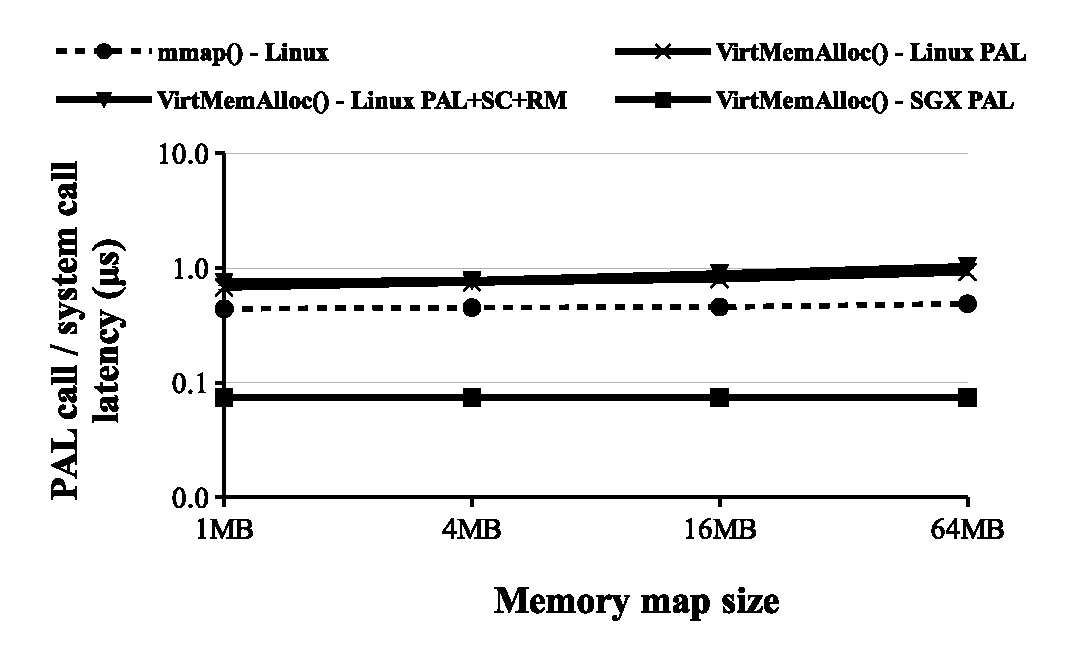
\includegraphics[height=10em]{pal/mmap-latency}
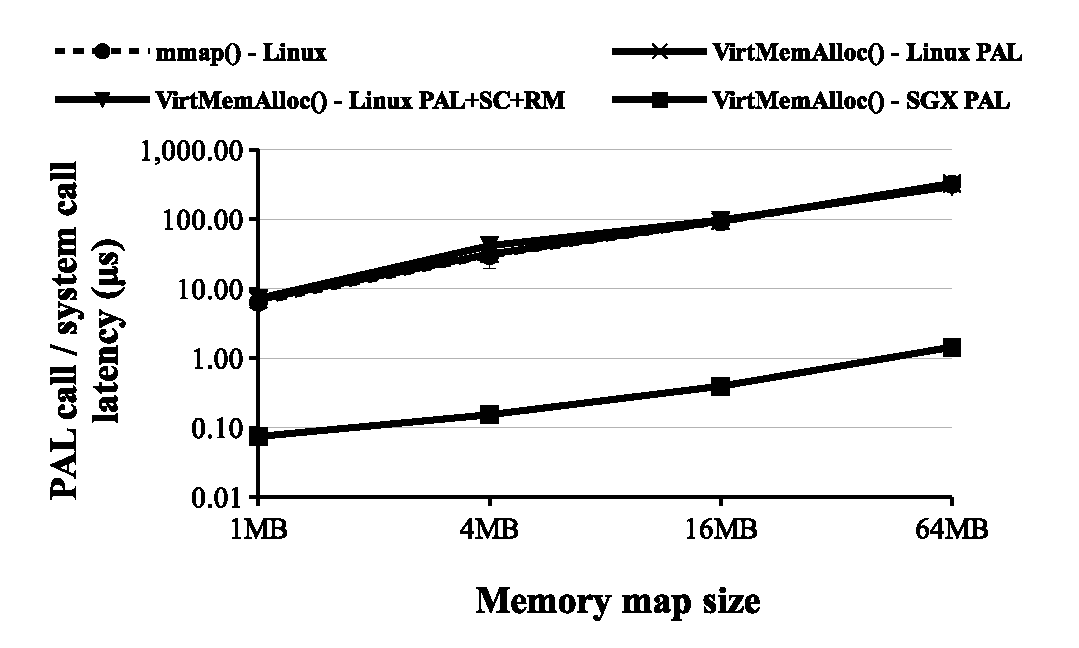
\includegraphics[height=10em]{pal/mmap-access-latency}
}
\parbox{0.49\textwidth}{\centering\bf (a) allocation + deallocation}
\parbox{0.49\textwidth}{\centering\bf (b) allocation + memory access + deallocation}
\caption{Latency of (a) allocating and deallocating a range of virtual pages, and (b) the same operations with writing to each page after allocation. Lower is better.
The comparison is between (1) \syscall{mmap} and \syscall{munmap} on Linux; (2) \palcall{VirtMemAlloc} and \palcall{VirtMemFree} on the Linux PAL, with and without a \seccomp{} filter ({\bf +SC}) and reference monitor ({\bf +RM}); (3) the same \hostapis{} on the SGX PAL, with and without zeroing the pages before use ({\bf +Zero}).}
\label{fig:eval:pal:mmap-latency}
\end{figure*}


Figure~\ref{fig:eval:pal:mmap-latency} (a)
shows that, if a \picoproc{} or a process simply allocate a range of virtual pages,
the latency is mostly constant,
except the minor cost of updating the page table
inside the host kernel.
On the Linux PAL, the overhead of translating \palcall{VirtMemAlloc} and  \palcall{VirtMemFree}
to \syscall{mmap} and \syscall{munmap}
is 50--80\%,
which mostly contributes to the checks for valid address mapping ranges, so that the guest cannot overwrite the memory used by the Linux PAL itself.
On the SGX PAL, the fundamental latency of allocating and deallocating virtual pages is extremely low,
because an enclave must preallocate the pages before initialization to maintain a static enclave signature.
The overhead of the \seccomp{} filter and reference monitor is marginal; especially since a \picoproc{} can only map pages internally, the reference monitor does not have to check any calls of \syscall{mmap} and \syscall{munmap}.
Theoretically, page allocation and deallocation
inside of an enclave should only involve updating
the records within the enclave memory.
However,
since SGX doesn't guarantee the initial state of the heap space inside an enclave,
the current design must zero the pages
after the allocation.
The latency of zeroing the pages can be several order-of-the-magnitude more expensive than
simply updating the page table,
and is proportional to the allocation size.



Figure~\ref{fig:eval:pal:mmap-latency} (b)
shows the latency of allocating and deallocating virtual pages
and writing to the beginning of each page in between allocation and deallocation.
In this experiment, the latency on the Linux PAL and the latency in a native Linux process
are both proportional to the allocation size,
ranging from 7\usec{} to 27\usec{} for allocating 1MB to 64MB memory.
Without zeroing the pages after the allocation,
the latency on the SGX PAL is still much lower than the Linux PAL and Linux, but becomes proportional
to the allocation size as well.
With page zeroing, the latency is close to the allocation and deallocation latency on the SGX PAL,
as shown in Figure~\ref{fig:eval:pal:mmap-latency} (a).







\subsection{Scheduling}
\label{sec:eval:pal:sched}

This section evaluates several \hostapis{} for scheduling several threads or processes
on a multi-core system,
including thread creation, polling I/O streams (TCP sockets for instance), and using several synchronization primitives,
such as notification events and mutexes. 


\begin{figure*}[t!]
\centering
\footnotesize
\resizebox{\textwidth}{!}{%
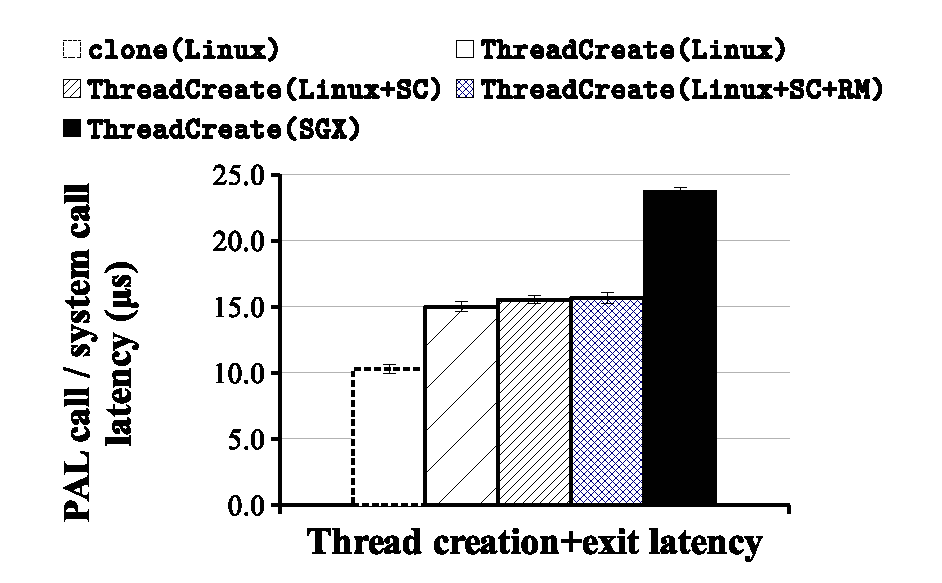
\includegraphics[height=10em]{pal/thread-latency}
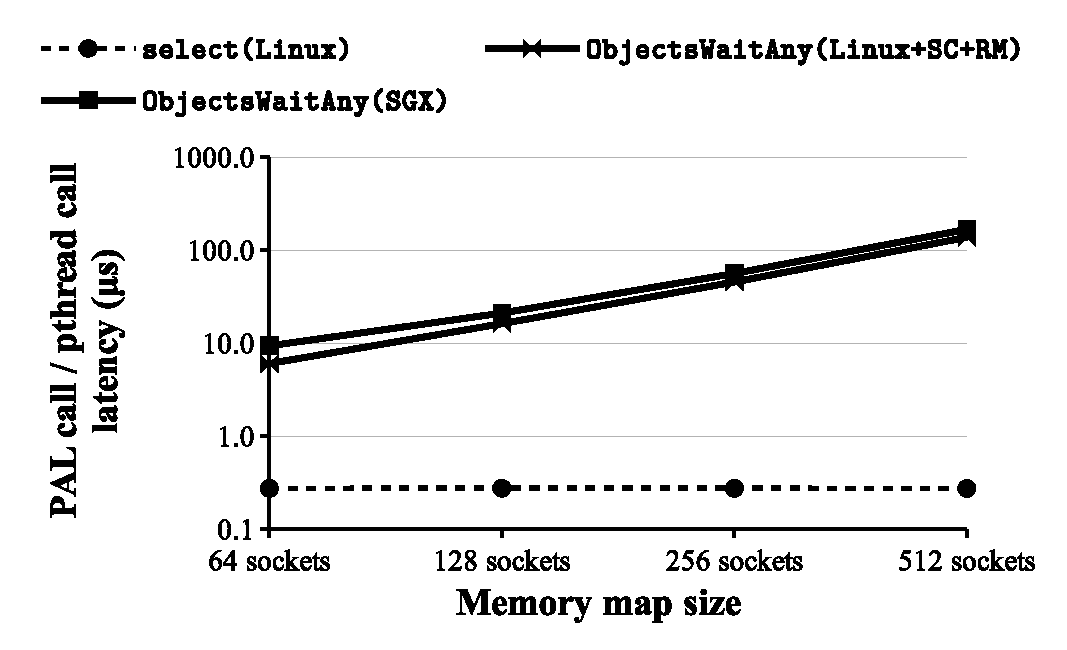
\includegraphics[height=10em]{pal/tcp-select-latency}
}
\parbox{0.49\textwidth}{\centering\bf (a) thread creation}
\parbox{0.49\textwidth}{\centering\bf (b) polling N TCP sockets}
\caption{(a) Thread creation latency and (b) latency of polling a number of TCP sockets.
Lower is better.
The comparison is between (1) \syscall{clone} and \syscall{select} on Linux; (2) \palcall{ThreadCreate} and \palcall{ObjectsWaitAny} on the Linux PAL, with and without a \seccomp{} filter ({\bf +SC}) and reference monitor ({\bf +RM}); (3) the same \hostapis{} on the SGX PAL.}
\label{fig:eval:pal:thread-select-latency}
\end{figure*}


\paragraph{Thread creation.}
The evaluation shows the latency of creating a new thread within the current process or \picoproc{}.
Figure~\ref{fig:eval:pal:thread-select-latency} (a)
evaluates the latency of creating a thread using \palcall{ThreadCreate} and waiting for the new thread to terminate immediately using \palcall{ThreadExit}.
The comparison is with the latency of \syscall{clone}
and \syscall{exit} in a native Linux process.
For the Linux PAL,
the latency of \palcall{ThreadCreate} and \palcall{ThreadExit} is \roughly{}46\% higher
than thread creation and exit on Linux,
and the overhead contributes
to allocating an initial stack for the new thread (\palcall{ThreadCreate} does not take an extra argument for specifying the stack address).
The evaluation also shows that the impact of the seccomp{} filter and reference monitor on the latency of thread creation is marginal (less than 5\%).

For the SGX PAL, the cost of thread creation is much higher.
Creating an enclave thread on the SGX PAL takes three primary steps: (1) creating an untrusted host thread (a pthread, specifically); (2) attaching the host thread to an unused TCS (thread control section); (3) entering the enclave and initialize its state.
As a result, thread creation on the SGX PAL is \roughly{}131\% slower than \syscall{clone} on Linux.




\paragraph{Polling stream handles.}
The evaluation shows the latency of polling among a number of TCP sockets for incoming messages.
Figure~\ref{fig:eval:pal:thread-select-latency} (b)
compares the latency of
\palcall{ObjectsWaitAny} for polling the status
of 64--512 TCP sockets,
with \syscall{select} on Linux.
The result shows that both the Linux and SGX PALs impose significant overheads on the latency of polling the TCP sockets,
for scanning an array of PAL handles and retrieving the associated file descriptors.
Whereas the latency of \syscall{select} on Linux is constant at \roughly{}0.3\usec{}, the latency of \syscall{ObjectsWaitAny} on the Linux PAL is proportional to the number of sockets being polled,
ranging from 3.2--29.1\usec{} for 64--512 sockets.
The latency on the SGX PAL is close to this result,
with a fixed cost at \roughly 2.7\usec{} for exiting the enclave.






\paragraph{Events and mutexes.}
Figure~\ref{fig:eval:pal:sched-latency} (a) shows the latency of using notification events in the Linux or SGX PAL
for synchronization among threads,
in comparison of similar pthread primitives running on Linux.
In general,
a POSIX multi-threaded program
uses a conditional variable and a mutex, both supported by the pthread library, for achieving the same semantics as a notification event.
When comparing with these pthread primitives,
the time difference between one thread signaling a notification event and another thread being waken up,
on the Linux PAL, is slightly cheaper, due to skipping the additional bookkeeping of the pthread library.
The cost of enabling the \seccomp{} filter and reference monitor is \roughly{}10\%.
For the SGX PAL, signaling a notification event is much slower.
The overhead on the SGX PAL
is \roughly{}130\% to the latency
on the Linux PAL,
and mostly contributes to the cost of exiting the enclave to call \syscall{futex}.



\begin{figure*}[t!]
\centering
\footnotesize
\resizebox{\textwidth}{!}{%
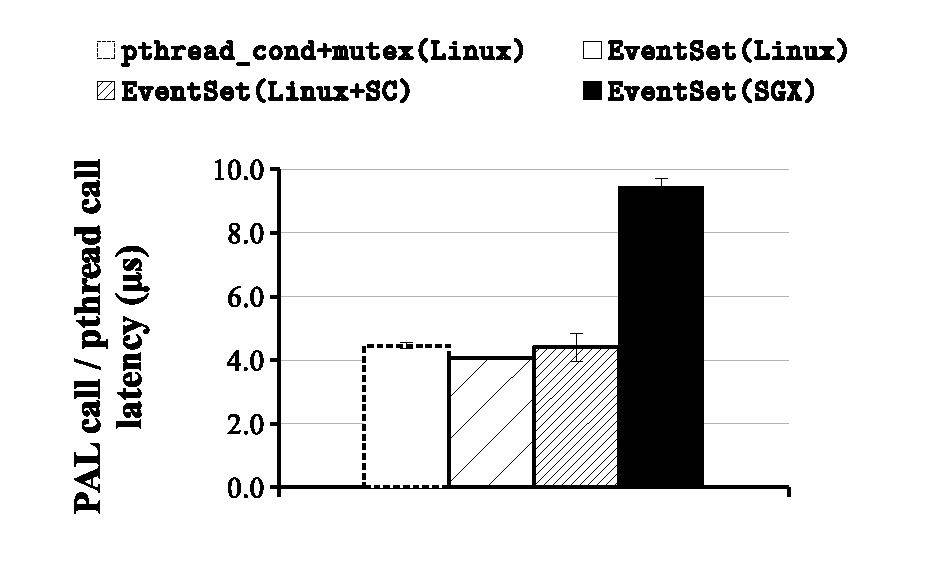
\includegraphics[height=10em]{pal/event-latency}
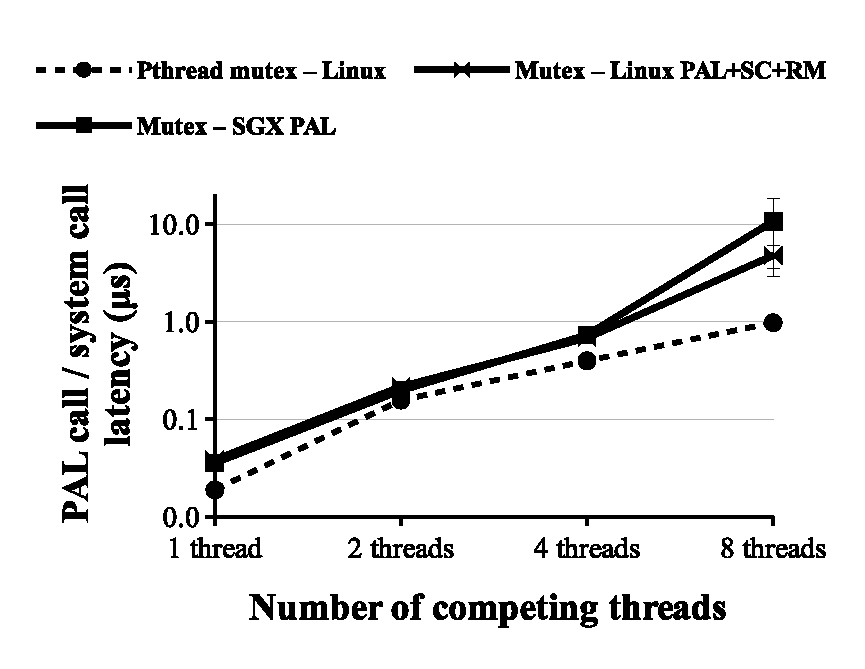
\includegraphics[height=10em]{pal/mutex-latency}
}
\parbox{0.49\textwidth}{\centering\bf (a) signal an event}
\parbox{0.49\textwidth}{\centering\bf (b) competing a mutex among N threads}
\caption{Latency of (a) signaling an event and (b) competing a mutex among N threads (N: 1 to 8).
Lower is better.
The comparison is between (1) pthread condition variables and mutexes on Linux; (2) Notification events and mutexes on the Linux PAL, with and without a \seccomp{} filter ({\bf +SC}) and reference monitor ({\bf +RM}); (3) the same abstractions on the SGX PAL.}
\label{fig:eval:pal:sched-latency}
\end{figure*}



Figure~\ref{fig:eval:pal:sched-latency} (b) shows the latency of acquiring and releasing a mutex.
With a single thread, the latency of acquiring and releasing a pthread mutex is \roughly{}0.02\usec{};
the latency of acquiring and releasing a PAL mutex,
on either the Linux PAL or the SGX PAL,
is \roughly{}0.04\usec{}, due to a slightly less optimized design than the pthread library of \glibc{}.
Either the Linux or SGX PAL does not invoke any \linuxapi{} or enclave calls
when a single thread accesses a mutex.
If multiple threads compete on a mutex, the latency grows roughly proportional
to the number of threads,
because each thread may block until other thread release the mutex.
Moreover, to avoid spinning on a mutex,
a process or \picoproc{} may forfeit the CPU to the holder of the mutex, using \syscall{futex}.
Because of the overhead of blocking and signaling using futexes,
with eight competing threads,
the average latency of acquiring and release a mutex
on the Linux PAL is 286\% longer than the latency of pthread mutex on Linux;
the average overhead on the SGX PAL
is much more expensive, at \roughly{}10$\times$.
 






\subsection{Multi-process abstractions}
\label{sec:eval:pal:multi-proc}

This section evaluates the performance of two multi-process abstractions in \thehostabi:
process creation and bulk IPC.



\paragraph{Process creation.}
Figure~\ref{fig:eval:pal:proc-latency}
shows the latency of process creation using \palcall{ProcessCreate}
and process exit
using \palcall{ProcessExit}.



The evaluation compares the process creation latency
with \syscall{vfork}, \syscall{execve}, and \syscall{exit},
which also create a clean process
and then terminate it.
To make a fair comparison,
the executable given to \syscall{execve}
is compiled as a static binary,
since the Linux PAL is also compiled as a static library.



Figure~\ref{fig:eval:pal:proc-latency} (a)
shows that the latency of process creation and exits on the Linux PAL, either with or without the \seccomp{} filter and reference monitor,
 


\begin{figure*}[t!]
\centering
\footnotesize
\resizebox{\textwidth}{!}{%
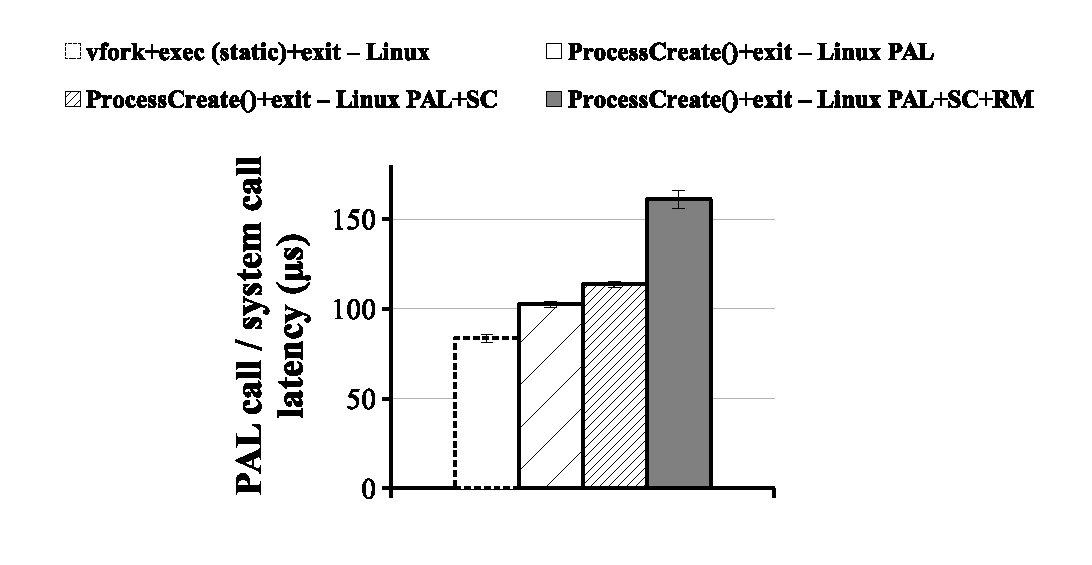
\includegraphics[height=10em]{pal/proc-latency}
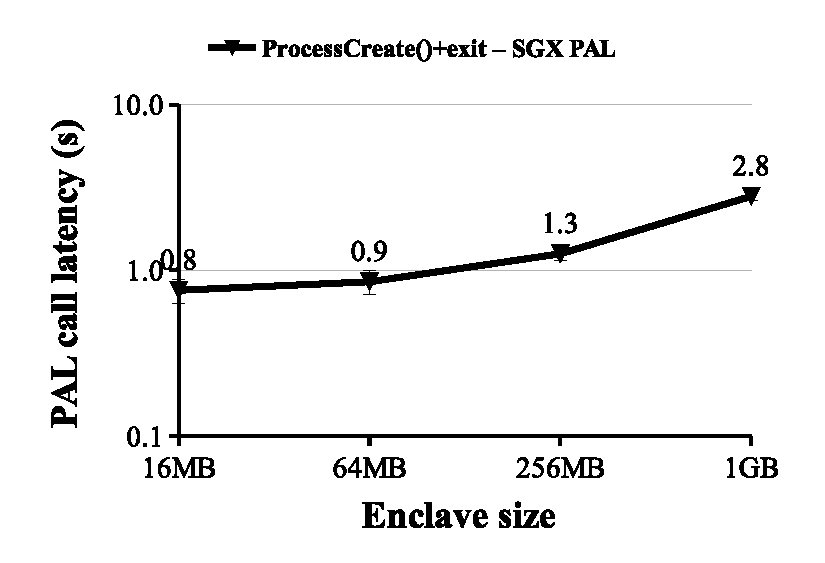
\includegraphics[height=10em]{pal/sgx-proc-latency}
}
\parbox{0.59\textwidth}{\centering\bf (a) process creation+exit}
\parbox{0.39\textwidth}{\centering\bf (b) SGX enclave creation+termination}
\caption{Latency of creating (a) a clean process on the Linux PAL, and (b) an enclave on the SGX PAL, in respect of different enclave sizes.
The comparison is between (1) a combination of \syscall{vfork} and \syscall{exec}'ing a minimal static program on Linux; (2) \palcall{ProcessCreate} on the Linux PAL, with and without a \seccomp{} filter ({\bf +SC}) and reference monitor ({\bf +RM}); (3) the same \hostapi{} on the SGX PAL.}
\label{fig:eval:pal:proc-latency}
\end{figure*}





\begin{figure*}[t!]
\centering
\footnotesize
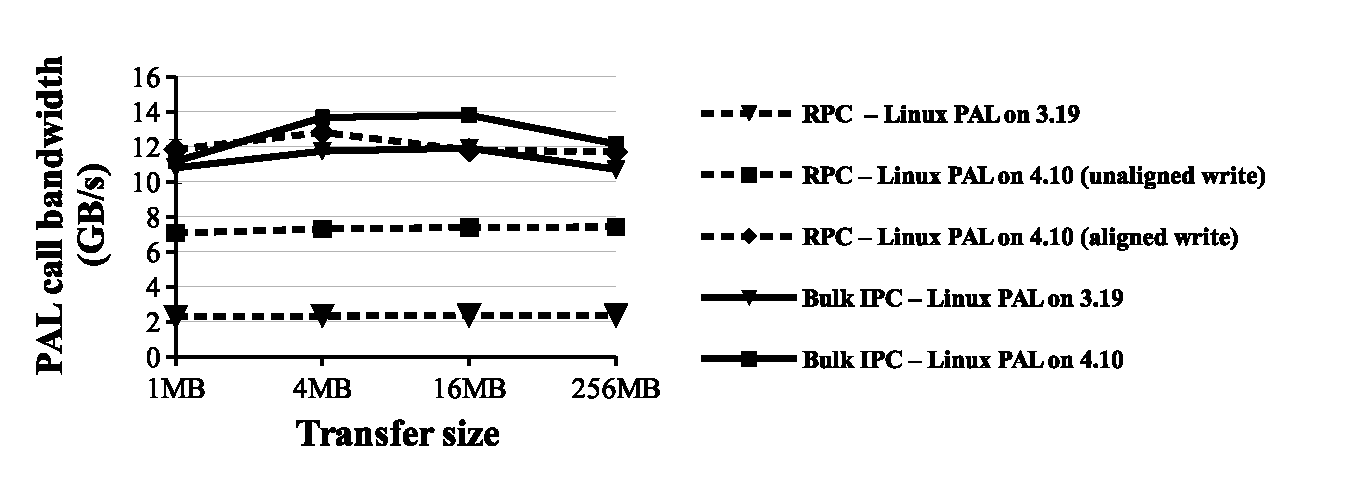
\includegraphics[width=.85\textwidth]{pal/gipc-bandwidth}
\caption{Bandwidth of sending large messages over (a) RPC streams and (b) Bulk IPC channels. The messages are sent in different sizes (1MB to 256MB), and either aligned or unaligned with the page boundary.
Higher is better. Both abstractions are benchmarked on Linux kernel 3.19 and 4.10 as the hosts. The impact of the \seccomp{} filter or reference monitor is marginal (less than 1\%).}
\label{fig:eval:pal:gipc-bandwidth}
\end{figure*}


\paragraph{Bulk IPC vs RPC streams.}




\subsection{Exception handling}


\begin{figure*}[t!]
\centering
\footnotesize
\resizebox{\textwidth}{!}{%
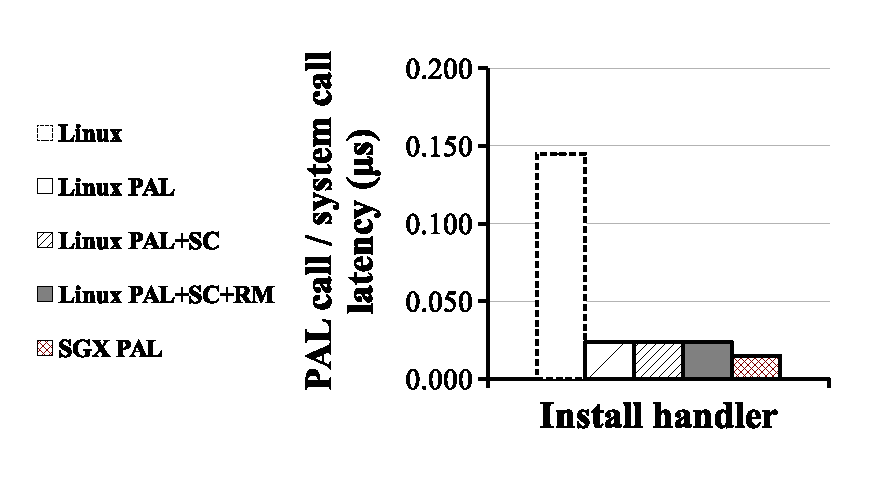
\includegraphics[height=10em]{pal/sig-install-latency}
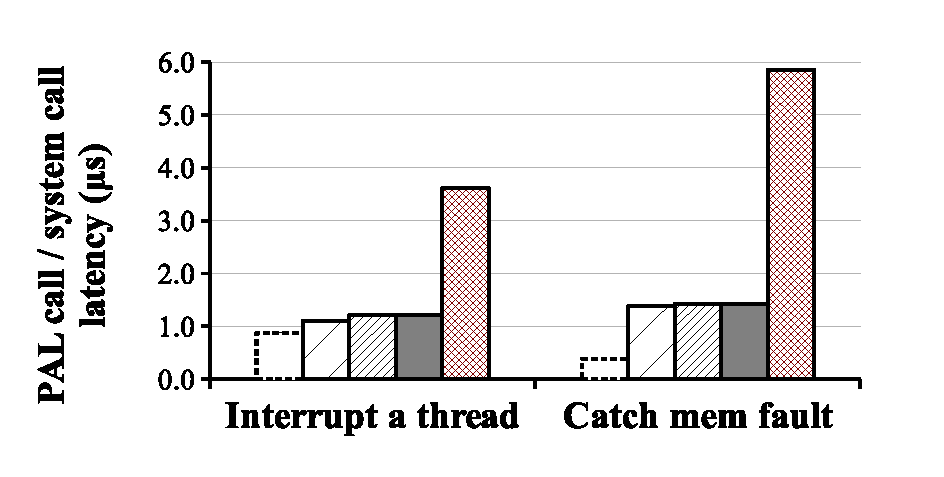
\includegraphics[height=10em]{pal/sig-catch-latency}
}
\caption{Latency of (a) installing an exception handler; (b)
interrupting a running thread with signals (on Linux) or \palcall{ThreadInterrupt} on the PALs; (c) catching a memory protection fault. Lower is better. The comparison is between (1) signals on Linux; (2) the Linux PAL, with and without a \seccomp{} filter ({\bf +SC}) and reference monitor ({\bf +RM}); (3) the SGX PAL.}
\label{fig:eval:pal:sig-latency}
\end{figure*}